\chapter{Analyses} % Main chapter title

\label{Chapter:Analyses}

As presented in Fig. \ref{fig:sustainableCityFramework}, the indicators for measuring a sustainable city are categorised into economic, social and environmental. This section of the paper discusses the nexus between urban agriculture and sustainable cities with reference to the indicator-sets under each of the themes.

\section{Urban agriculture and economic sustainability of cities}

\subsection{Full-time employment}

Urban agriculture provides employment, and has thus become a major means of livelihood, for people in many cities particularly in the global south (Darkey et al., 2014; Zezza \& Tasciotti, 2010). An estimated 2100 farm labourers in Morogoro and 6400 in Mbeya, Tanzania are engaged in urban agriculture as either attendants or fodder collectors (International Labour Organization, 2013). Similarly, approximately 120,000 low-income households (including farmers, garland makers and garland sellers) in Manila, Philippines depend on jasmine production for their livelihoods (IPC, 2007). Many examples of urban agriculture's role in employment creation abound in the conventional literature (see: Amponsah et al., 2015a; Carr, Potter, \& Nortcliff, 2011; Sinclair, 2010; Tiongco, Narrod, \& Bidwell, 2010). The general observation is that urban agriculture's role in employment creation is widespread in the global south as depicted in Table \ref{tbl:peopleEngagedInUA}.

\begin{table}[th]
\caption{Number of people engaged in urban agriculture in the global south. Source: FAO (2007).}
\begin{center}
\begin{tabular}{ p{0.20\textwidth} p{0.25\textwidth} p{0.45\textwidth} } 
\hline
Region & Number (million) & Principal live-hood \\
\hline
Sub-Saharan Africa & 11 & Commercial vegetable growing or dairy farming \\
Northern Africa and the Middle East region & 6 & Horticultural and livestock products (fruit, vegetables and poultry) \\
South Asia & 11 & Perishable high-value commodities such as milk and fresh vegetables \\
East and South-East Asia & 7 & Perishable high-value commodities such as milk and fresh vegetables \\
\hline
\label{tbl:peopleEngagedInUA}
\end{tabular}
\end{center}
\end{table}

Not only is urban agriculture a source of employment to farmers but also to stakeholders along the value chain (Fig. \ref{fig:vegySupplyChain}). Community and farmers' markets and door-to-door delivery of food baskets in Argentina, Brazil and Uruguay are examples of jobs created in the commercial sector by urban agriculture (International Labour Organization, 2013). Similarly, majority of vegetable farmers in urban and peri-urban Ghana deliver their produce to wholesalers, who are predominately women, at the farm-gate (Abaidoo et al., 2009; Amoah, Drechsel, Henseler, \& Abaidoo, 2007; Amponsah et al., 2016). These wholesalers in turn sell the produce to retailers, food vendors and households as depicted in Fig. \ref{fig:vegySupplyChain}. The farm produce is conveyed from the farm-gate to the open markets by transport operators.

\begin{figure}[th]
\centering
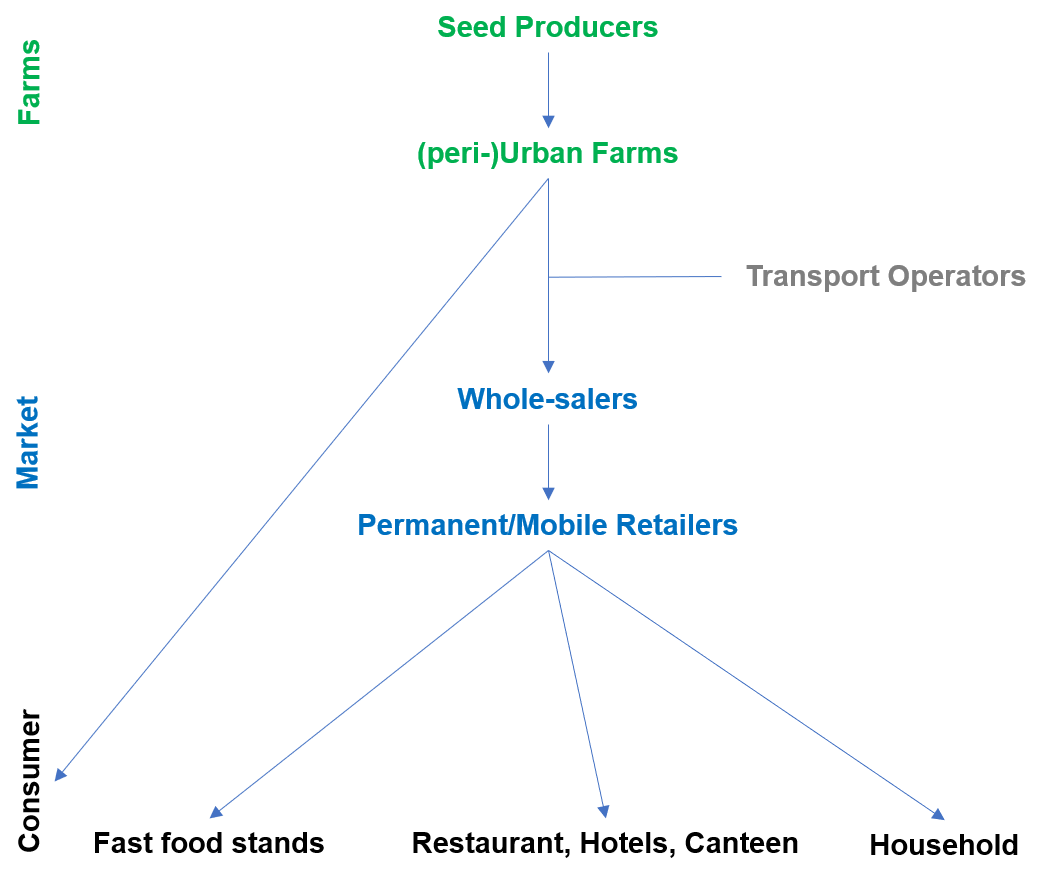
\includegraphics[width=0.75\textwidth]{./Figures/vegySupplyChain.png}
\decoRule
\caption[Carbon Nano-wires Fabrication Process]{Fabrication process of carbon nano-wires to achieve through the proposed dissertation.}
\label{fig:vegySupplyChain}
\end{figure}

The discussion so far suggests that urban agriculture makes a profound contribution to the employment of the labour force in the global south. The situation differs from the cities in the global north because the narrative in the conventional literature suggests that the motivation for urbanites and city authorities to promote agriculture in these cities lies in its ecological functions as well as its support for leisure and recreation (Pearson et al., 2010). The implication is that the role of urban agriculture in employment creation in the global north may not be as profound as it is in the global south. This is because, urban agriculture in the global north is not economically-centred but rather centred on its environmental functions. Nonetheless, recent studies give indications that the functions of urban agriculture in the global north is gradually shifting from leisure and recreation to more of urban sustainability and economic resilience (Lovell, 2010; McClintock, 2010). The increasing focus on economic resilience means that the contribution of urban agriculture in the global south and north appears to be converging even though there are variations across cities. Nevertheless, if the agricultural lands had been used for non-agricultural purposes, the employment effects may have been more profound. For instance, industrial and commercial activities on these parcels of land may have made more profound contributions to employment creation.

\subsection{Employment for women}

According to Prain and Lee-Smith (2010), two out of every three urban farmers in Yaounde, Nakuri, Maputo, Nairobi and Kampala are women. Generally, these women farmers engage in subsistence farming with the objective of meeting the family demand for fresh, nutritious and chemical-free food (Gamhewage, Sivashankar, Mahaliyanaarachchi, Wijeratne, \& Hettiarachchi, 2015). The rest of the urban women farmers sell the excess produce for income. However, agriculture could be a burden to these women due to the numerous roles they perform at the household level. The argument does not pertain to agriculture but also applies to almost all the economic activities the women are engaged in. The implication is that without addressing the issues that foster gender inequality, women's engagement in agriculture in the cities could be a burden (Veenhuizen, 2006). There must therefore be a conscious effort by policy makers and social advocates to help minimise the pressure on women emanating from the combination of household chores and economic activities such their involvement in urban agriculture.

Generally, commercial urban agriculture is dominated by men as depicted in Table \ref{tbl:genderinUA}. In contrast, women are dominant at the market and food vending stages of the supply chain (Drechsel \& Keraita, 2014). It can therefore be deduced that commercial agriculture in the cities in the global south is gendered and thus makes a profound contribution to employment for both women and men. However, as the economic arguments have always been, if the agricultural lands were used for nonagricultural purposes, more women may have been employed. This argument lies at the heart of the theory of ‘highest and best use’ of urban land.

\begin{table}[th]
\caption{Gender in urban agriculture in selected cities. Source: Drechsel et al. (2006).}
\begin{center}
\begin{tabular}{ p{0.20\textwidth} p{0.40\textwidth} p{0.15\textwidth} p{0.15\textwidth} } 
\hline
Country & City & Female (\%) & Male (\%) \\
\hline
Benin & Cotonou & 25 & 75 \\
Burkina Faso & Ouagadougou & 38 & 62 \\
Cameroun & Yaoundé & 16 & 84 \\
Cote d'Ivoire & Abidjan/Bouake & 5-40 & 60-95 \\
Gambia & Banjul & 90 & 10 \\
Ghana & Accra, Kumasi, Takoradi and Tamale & 10-20 & 80-90 \\
Guinea & Conakry, Timbi-Madina & 70 & 30 \\
Mali & Bamako & 24 & 76 \\
Mauritania & Nouakchott & 15 & 85 \\
Nigeria & Lagos/Ibadan & 5-25 & 75-95 \\
Sierra Leone & Freetown & 80-90 & 10-20 \\
Togo & Tsévié, Lome & 20-30 & 70-80 \\
India & Delhi, Mumbai, Chennai, Hyderabad and Bengaluru & 17 & 83 \\
\hline
\label{tbl:genderinUA}
\end{tabular}
\end{center}
\end{table}

\subsection{Income generation and gross domestic product}

Several households in both developing and middle income countries opt for urban agriculture as a source of livelihood (Abaidoo et al., 2009; Foeken \& Owuor, 2008; Raschid-Sally \& Jayakody, 2008a). Drechsel and Keraita (2014) point out that two out of every three urban vegetable farmers in Accra, Ghana had no intentions of leaving the job even if they were offered regular salaried employment. Based on this and many other factors (such as limited employment opportunities in the formal sectors, flexibility in work schedules, etc.), Amponsah et al. (2015b) conclude that vegetable farming in Kumasi, Ghana's second largest city, had become an employment destination for many.

Amponsah et al. (2015b) conclusion could be attributed to the higher incomes the farmers earned from the agricultural activities in the cities. For instance, Keraita, Jiménez, \& Drechsel (2008) identified that urban farmers in Ghana earned twice or more the incomes of their counterparts in rural areas. This appears to be the case in several other cities in the global south as indicated in Table \ref{tbl:incomesByUfarmens}. The earnings enable the urban farmers to contribute to national income. For instance, YiZhang and Zhangen (2000) found that 2.7 million urban farmers contributed 2\% of Shanghai's gross domestic product. Similarly, para grass production and sale in Hyderabad, India contributes an estimated annual income of USD 4.5 million to the city's economy. In Hartford, USA, urban agriculture is estimated to contribute between 4 and 10 million dollars in gross domestic product (Nugent, 1999).

\begin{table}[th]
\caption{Incomes earned by urban vegetable farmers in six cities. Source: Ensink et al. (2004); Buechler \& Devi (2005); Drechsel et al. (2006); Keraita, Jiménez, \& Drechsel, 2008.}
\begin{center}
\begin{tabular}{ p{0.30\textwidth} p{0.30\textwidth} p{0.30\textwidth} } 
\hline
City & Annual income per ha (US\$) & Annual GNI per capita (US\$) \\
\hline
Nairobi in Kenya & 1770 & 645 \\
Dakar in Senegal & 2234 & 773 \\
Kumasi in Ghana & 420-1920 & 522 \\
Hyderebad in India & 830-2800 & 771 \\
Haroonabad in Pakistan & 840 & 931 \\
Guanajuato in Mexico & 1935 & 7755 \\
\hline
\label{tbl:incomesByUfarmens}
\end{tabular}
\end{center}
\end{table}

The value of urban agriculture to a city's gross domestic product may not be significant when compared to non-agricultural land uses. This could be a justification for the pricing out of agriculture in city land use planning processes. However, as indicated earlier, gross domestic production and other economic indicators underestimate the actual contribution of urban agriculture to city development. The approach excludes ecological and social dimensions of urban agriculture. Probably, if these dimensions could be valued and added to the value of urban agriculture, then urban agriculture could be as valuable as other land uses.

\subsection{Savings and expenditure}

A study by Prain and Lee-Smith (2010) revealed that households who consumed the produce from their farms in Kampala in Uganda and Yaounde in Cameroon were able to save part of their incomes. Once individuals farm on their own, there is no need to spend money to buy some agricultural commodities. On this basis, Smit, Nasr, \& Ratta (2001) maintains that households who engaged in farming in cities in Zambia saved between 10 and 15\% of food costs. Furthermore, studies in Bangalore, Nairobi, Lima and Accra revealed that savings coming from own food production enabled households to purchase other types of food (World Bank, 2013). For instance, households in Bangalore were able to save between 1.30 and 80.00 USD per month (World Bank, 2013) whereas farmers in the cities in Kenya were able to save between 7 and 14 USD per month (Freeman, 1993). These savings are spent on other household items that contribute to improved quality of life.

It can be observed from Table \ref{tbl:expenditurePattern} that expenditure on food in Bangalore, Accra and Nairobi for households who engaged in urban agriculture was below the average of 50–70\% for the urban poor (FAO, 2007). The situation in the cities in the global north may be different given that urban households are driven by leisure and recreation to engage in agriculture cites. In these cities, households spend minimum proportions of their incomes on food, which implies limited contribution of urban agriculture to household savings. The savings may however originate from transportation. The literature indicates that households spend less on transport to obtain or transport food as compared to the other household items. Hamilton et al. (2013) had earlier observed that savings occurred as a result of the reduction in transport cost for the urban farmer. The savings result from the amount these farmers would have otherwise incurred if they were to travel to procure the items, they produce themselves. Furthermore, urban agriculture means some farm produce are now closer to consumers than if the produce were to be supplied by rural farmers. This will therefore reduce travel cost and time to access food items by urban dwellers.

\begin{table}[th]
\caption{Expenditure pattern of urban agriculture households in some selected cities. Source: World Bank (2013).}
\begin{center}
\begin{tabular}{ p{0.30\textwidth} p{0.20\textwidth} p{0.20\textwidth} p{0.20\textwidth} } 
\hline
Expenditure item & Selected cities &  &  \\
  & Bangalore & Accra & Nairobi \\
\hline
Food & 29.2 & 36.5 & 39.4 \\
Utilities & 16.8 & 12.3 & 13.1 \\
Education & 11.5 & 16.7 & 16.9 \\
Health & 10.4 & 8.2 & 5.1 \\
Clothes & 8.1 & 7.7 & 3.0 \\
Shelter & 7.0 & 3.2 & 18.9 \\
Loan/debt & 6.2 & 1.4 & 0.4 \\
Transport & 4.6 & 7.9 & 2.5 \\
Other & 3.3 & 0.8 & 0.2 \\
Family events & 2.1 & 4.5 & 0.2 \\
Domestic help & 0.7 & 0.8 & 0.2 \\
\hline
\label{tbl:expenditurePattern}
\end{tabular}
\end{center}
\end{table}

\subsection{Tax revenue}

Taxes are very important elements in managing developmental activities in cities. Taxes collected through urban agriculture covers all the actors along the produce supply chain. It is worth noting that, national income from taxes from urban agriculture can be directly linked to the expenditure farmers make and the employment obtained.

Property taxes have been identified as a city's main source of income (World Bank, 2015). Urban agriculture contributes significantly to tax revenues from property taxes. According to Liu (2008) and Voicu and Been (2008), urban farms and community gardens contribute to the increase in home values. For instance, the presence of gardens in California contributed to the rise in property values as much as 9.4% within five years of establishment (Voicu & Been, 2008). The revenues were estimated at half a million dollars per garden over twenty years.

Transportation taxes are also paid by urban farmers who transport their goods within or outside the urban area. Some urban farmers indirectly pay transportation taxes through the purchase of fuel for irrigation or the transportation of farm goods and services. Additionally, the wholesalers or retailers engaged in the sale of the urban agricultural produce pay taxes to city authorities. In Kumasi, a city in Ghana, wholesalers and retailers who operate in the open markets pay taxes in the form of market tolls (tickets) (Baah-Ennumh \& Adom-Asamoah, 2012). The amounts paid ranges from 5 to 10GHp (0.01 USD–0.02 USD) a day and are paid to the Kumasi Metropolitan Assembly. Similarly, in the United States, the income that is obtained from urban farming does not represent a separate kind of income. They are determined and taxed like income from other businesses of a comparable size apart from some detailed regulations regarding farm income. However, national subsidies for soil, groundwater or environmental protection, care for wild animals or forests are sometimes tax-free for the farmers (Andersen, Asheim, Mittenzwei, \& Veggeland, 2002). In a similar vein, some municipalities (Rosario in Argentina and Cagayan de Oro in The Philippines) use tax exemptions as a means of promoting urban agriculture.

Useful as the taxes may be, taxes to the cities may be more if the agricultural lands had been used for non-agricultural purposes such as commerce or industry. The tax exemptions could also be avoided if the lands were used for non-agricultural purposes. Such arguments are underpinned by the theory of ‘highest and best use’ which focuses on only the direct economic benefits derived from the use of land. These theories suggest that allocating land for urban agriculture deprives its access for other more economically beneficial uses such as industrial, commercial and residential uses. This explains why a rise in the value of urban agricultural land is mostly associated with the change in use from agriculture to alternative land uses (Nugent, 2000).

\section{Urban agriculture and social sustainability of cities}

\subsection{Educational functions}

Golden (2013) suggests that urban agriculture provides a medium for learning experiences, youth development and educational programmes. Agricultural projects in California and Philadelphia in the United States of America are used to highlight the role of urban agriculture in education (Bradley \& Galt, 2014; Ober Allen, Alaimo, Elam, \& Perry, 2008; Travaline \& Hunold, 2010). These educational services are directed towards teaching the citizens where, how and by whom the food they eat is grown so as to enable them make informed decisions about their food systems. The agricultural projects in the cities serve as avenues for children and adults to acquire practical skills on food production and processing.

Furthermore, through their social networks, urban farmers who have had the benefits of education by research institutions impart the knowledge to their counterparts. For instance, urban vegetable farmers in Kumasi in Ghana who have participated in research activities on the World Health Organization's Multiple Barrier Interventions have transferred the knowledge to their counterparts who were not part of the training programme (Amponsah, Vigre, Schou, Braimah, \& Abaidoo, 2015a). This is used to highlight the replication effects of such research projects on the larger community.

Urban farmers' earnings from agriculture are used to support their children in school (Prain \& Lee-Smith, 2010). A study conducted in SriLanka by Gamhewage et al. (2015) concluded that 22\% of urban farmers prefer to expend their savings on the education of their children to spending on household possessions. Similarly, in India, some women contribute approximately 23\% of their share in household education expenditure from the incomes they earn from urban agricultural activities. Another study in Kampala, Uganda also concluded that urban male farmers and female farmers spend 26\% and 12\% of their incomes respectively on the fees of their wards in school (Devi \& Buechler, 2009).

Nevertheless, urban agriculture, particularly in the global south, is known to fuel child labour and truancy in school (Edet \& Etim, 2013; International Labour Organization, 2006). For instance, in Dar es Salaam, Tanzania, children have been found to engage in urban agriculture at the expense of their education. Similarly, child migrants have been found to be engaged as farm labourers on urban farms in Kumasi, Ghana (Amponsah et al., 2016). Yet, in these countries, child labour is prohibited. The higher returns from the urban agricultural activities could be an explanation for their attractiveness to children, especially migrant children.

By enforcing the child labour laws, the children can take advantage of the free and compulsory universal primary educational policies and programmes in these countries to enrol in schools (Nishimura \& Yamano, 2013; Rodeghier, Hall, \& Useem, 1991). This will ultimately enhance the educational functions of urban agriculture towards social sustainability of cities.

\subsection{Civic engagement}

A growing body of literature points to the increasing importance of community supported agriculture in civic engagements. For instance, Obach and Tobin (2014) and Pole and Gray (2013) found that people in New York City who were engaged in urban agriculture were more politically engaged and more likely to volunteer in their communities compared to the general population. Similarly, in Dar es Salaam in Tanzania, urban farms were used as political gathering spaces in the run up to the 2010 elections. In fact, some farms had small concrete platforms that were used for political rallies. Despite these observations, Pole and Gray (2013) maintain that generally, the desire for organic foods is the motivation for people to interact with urban farmers other than civic engagement. Obach and Tobin (2014) add that consumers of urban agricultural produce are less likely to engage in charitable giving than the general population. The authors conclude that if the motivation for engaging in urban agriculture is economic, then it is less likely to promote civic engagement.

The narrative points out that economic reasons including household food security, employment and income generation are the main motivations for people's engagement in urban agriculture (Abaidoo et al., 2009; Amoah et al., 2007; Amponsah et al., 2016; Darkey et al., 2014; International Labour Organization, 2013; Zezza \& Tasciotti, 2010). On the other hand, the reasons for agriculture in the cities in the global north are more inclined towards leisure and ecological functions (Hamilton et al., 2013; International Labour Organization, 2013; Walker, 2015). In this regard, urban agriculture's role in civic engagement may be more pronounced in the global north than the global south.

\subsection{Safety and security}

Urban agriculture makes an important contribution to the safety of a city. For instance, roof-top gardens help to promote energy efficiency in buildings and contribute to fire prevention (Hoornweg \& Munro-Faure, 2012; Rashid \& Ahmed, 2011; Wong et al., 2003). Furthermore, clearing an area of bush in a city for agricultural purposes has the potential to eliminate hiding spaces for thieves (real or imagined). Customers, people walking through, people who live nearby, people looking for a day labour job, and more, all interact with urban farmers. The interactions make profound contributions to the social sustainability of cities.

A study by the University of Pennsylvania's Perelman School of Medicine in Philadelphia found that greening vacant lots (which could take the form of urban agriculture) made nearby residents feel significantly safer, and that the greened lots were linked to reductions in certain gun crimes in the area (Krauser, 2012). This is consistent with the results of the work of Kuo and Sullivan (2001) which revealed that the greener a building's surroundings were, the fewer the reported crimes. Following this, the Youngstown Neighbourhood Development Corporation initiated a ‘Lots of Green’ programme in 2010 to reuse vacant lands. A recent study established that there were reductions in burglaries around stabilisation lots, and assaults around community reuse lots (Kondo, Hohl, Han, \& Branas, 2016). This could be a validation of the broken window theory, which states that maintaining and monitoring urban environments in a well-ordered condition may stop further vandalism and escalation into more serious crime. The Urban Food Crisis (2018) explains that using blighted lots for urban agricultural purposes sends a signal that criminal activities are not welcome in the area, which ultimately reduces crime rates.

Other studies point to the negative side of urban green space (Bixler \& Floyd, 1997; Ulrich, 1993; Van den Berg \& Ter Heijne, 2005). These include encounters with physical danger such as poisonous animals and thorny plants, and the fear of crime (Sreetheran \& van den Bosch, 2014). These authors, after a systematic review of literature, point out, however, that factors such as gender and individual's experiences are most influential in evoking fear of crime. This means that the crimes that result from urban agriculture may be imagined from an earlier experience. A fear of crime may therefore be imagined but not real. People should be alerted to thorny plants and poisonous animals to mitigate the adverse effects on neighbourhoods. These measures could enhance the role of urban agriculture in urban safety and security.

\subsection{Gender equality and social equity}

Urban agriculture contributes to bridging gender gap and promotes social equity through the employment opportunities it offers to both men and women. As presented earlier in Table 2, women form a significant part of the labour force that is engaged in urban agriculture. They can gain employment at every stage of the supply chain. This reduces gender inequalities (Eigenbrod \& Gruda, 2015; International Labour Organization, 2013). A study conducted in Kisumu in Kenya by Mireri (2013), concluded that the proportion of male family labour engaged in urban agriculture is slightly higher (53\%) than that of women. However in the case of hired labour, more women (54\%) than men were employed. Kutiwa, Boon, and Devuyst (2010) also point out that urban agriculture in Harare in Zimbabwe provides women the opportunity to earn secondary income, improve nutritional value of the household diets, and participate actively in budgeting and decisionmaking processes at the household level. Similarly, both men and women are engaged in mushroom production, horticulture, aquaculture and livestock farming in Accra in Ghana (World Bank, 2013). These cases reveal that urban agriculture contributes to bridging the gender gap, which has positive implications for social equity.

However, women tend to engage in urban agriculture for household food supply while men engage in it for economic reasons. This could perpetuate the income gap between men and women in many cities. Furthermore, the disparity in the gender roles at the family level implies greater burden on women in the cities in the global south than men. Typically women shoulder more household responsibilities (like childcare and domestic work) than men (Lachance-Grzela \& Bouchard, 2010; Mencarini \& Sironi, 2012), which implies that urban agriculture could have the potential to aggravate the burden of work on women and gender inequality (Veenhuizen, 2006). These have implications for the systems and practices that perpetuate gender inequality but not necessarily preventing a certain gender category from engaging in urban agricultural activities or any economic activities.

\subsection{Health benefits}

Urban agriculture contributes to the health of a city through its contribution to food security (Golden, 2013; Opitz et al., 2016; Twiss et al., 2003; World Bank, 2013) and income for farmers and their families to access health care. Community gardens give residents access to fresh fruits and vegetables (Larsen \& Gilliland, 2009; Park et al., 2011), which are critical to safeguarding their health and that of the city in general. From a social point of view, urban agriculture can ensure food availability and accessibility, which can translate into food affordability. Also, women take advantage of the produce from household gardens to diversify the family food intake, which ultimately results in healthier diets. Research also shows that people who participate or have family members that engage in community gardens “were 3.5 times more likely to consume fruits and vegetables at least 5 times per day than people without a gardening household member” (Alaimo, Packnett, Miles, \& Kruger, 2008). In this regard, urban agriculture helps to reduce malnutrition and promote the general health of the city population.

However, some studies point to the adverse effects of urban agriculture on the health of the cities. These studies highlight the excessive use of agro-chemicals (Obuobie et al., 2006; Veenhuizen, 2006; Yamusa, 2014), which could undermine the health of producers, consumers and environment at large, and the use of untreated wastewater for food production without regard to safe practices in many cities in the global south (Amponsah, Vigre, Schou, Braimah, \& Abaidoo, 2015a; Becerra-Castro et al., 2015; Mara \& Sleigh, 2010; Ndunda \& Mungatana, 2013; Veenhuizen, 2006). In addition, the urban agricultural farms can result in the spread of diseases through mosquitoes and the scavenging animals.

Based on these adverse effects, the emphasis of the discourse on the role of urban agriculture in cities' social sustainability should focus on responsible agriculture. This underscores the need to regulate the urban agricultural subsector for compliance with safe agricultural practices and general neighbourhood sanitation measures.

\subsection{Recreation}

Community gardens and rooftop gardens contribute to both indoor and outdoor recreation (see Hamilton et al., 2013; Walker, 2015). These gardens can provide a place where people in an area in a city come together for mutual benefits. For instance, in the early 20th Century, upper class Russians resorted to dachas as hobby farming to improve upon recreation (Hamilton et al., 2013). Community gardens and rooftop garden also serve as tourist attraction centres (International Labour Organization, 2013) and improve the value of urban property. A classic example of this is in Beijing China. Here, people spend one-day to tour over 1900 sightseeing farms and pick produce (International Labour Organization, 2013).

Some individuals in Detroit have resorted to urban agriculture as a means of increasing the value of their property (Walker, 2015). Each community garden in California also contributed about half a million dollars to the local economy through rise in the value of real property (Voicu \& Been, 2008). People are attracted to some of these buildings because of the plants and ornaments around. It is on the basis of this that the World Bank (2013) suggest that countries should consider integrating urban agriculture into urban greening as a means to improving recreation, aesthetics and property values in their cities.

\subsection{Technology and innovation promotion}

Urban agriculture provides the avenue for the development of technology. For instance, some urban farms in Hong Kong Island, China are recycling water with PV-powered UV-LED disinfection (Close, Ip, \& Lam, 2006). Other farms use hydroponic (Buehler \& Junge, 2016; VOA News, 2016; Woodford, 2018), film farming (Joe, 2017) and aeroponic (Vyawahare, 2016) systems to produce leafy greens, tomatoes, and herbs. These technologies could contribute to the preservation of urban agriculture and its significant roles even in cities where land is increasingly becoming scarce due to rapid urbanisation.

Urban agriculture also provides an avenue for new research and technology to be developed. Examples include research on varieties of seeds, and type and amount of light required for plant growth. This type of agriculture therefore incorporates the use of technology as a means of optimising levels of production. Disregarding technology and innovation in urban agriculture could result in unreliable and ineffective farms.

\section{Urban agriculture and environmental sustainability of cities}



%\begin{figure}[th]
%\centering
%
\includegraphics[width=0.95\textwidth]{./Figures/FabricationProcess.png}
%\decoRule
%\caption[Carbon Nano-wires Fabrication Process]{Fabrication process of carbon nano-wires to achieve through the proposed dissertation.}
%\label{fig:fabricationFlowChart}
%\end{figure}

%\begin{equation}
%\left(\tau _t^e-\frac{\tau _n^e \text{dr}}{\text{dz}}\right) 2 \pi  r+\frac{d \left(\pi  r^2
%   \left(\tau _{\text{zz}}-p\right)\right)}{\text{dz}}+\frac{\gamma  \text{dr} 2 \pi  r}{r
%   \text{dz}}+\rho  g \pi  r^2=\frac{d \left(\rho  \pi  r^2 v^2\right)}{\text{dz}}
%\label{eq:linearMomentum}
%\end{equation}